\chapter{Приложения}
\label{ch:appendix}

    	
\section{Приложение А. Вывод расчётных формул и методика эксперимента}

    Температура измеряется термометром сопротивления. 

    \begin{equation}
        T(R_T) = 273 + \frac{R_T}{\alpha R_{\text{к}}} \left[ 1 + \alpha (T_{\text{к}} - 273) \right] - \frac{1}{\alpha}
        \label{T_R_T}
    \end{equation}

    Формула (\ref{T_R_T}) позволяет легко пересчитать кривые $R_{heat}(t)$, $R_{cool}(t)$ в кривые $T_{heat}(t)$, $T_{cool}(t)$. Входящий в формулу температурный коэффициент сопротивления меди равен $\alpha = 4.28*10^{-3} {\text{град}}^{-1}$.

    Из полученных ранее выражений, интегрированием, получается следующее:
    
    \begin{equation}
        \frac{-C}{\lambda} ln \frac{T_{cool} - T_{\text{к}}}{T - T_{\text{к}}} = t
        \label{eq:diff_integral}
    \end{equation}

    Откуда получается явная зависимость от времени:

    \begin{equation}
        T_{cool}(t) = (T - T_{\text{к}}) e^{\frac{- \lambda}{C} t} + T_{\text{к}}
        \label{T_cool_t}
    \end{equation}

    Уравнение (\ref{T_cool_t}) легко спрямляется в координатах ($ln \frac{T_{cool} - T_{\text{к}}}{T - T_{\text{к}}}$, $t$). Тангенс угла наклона данной прямой позволяет определить отношение искомых величин $\frac{\lambda}{C}$.

    Аналогично для прямой $T_{heat}$:

    \begin{equation}
        \frac{-C}{\lambda} ln \frac{P - \lambda (T_{heat} - T_{\text{к}})}{P} = t
        \label{eq:diff_integral2}
    \end{equation}

    Находим явную зависимость от времени:

    \begin{equation}
        T_{heat}(t) = \frac{P}{\lambda} (1 - e^{\frac{-\lambda}{C} t}) + T_{\text{к}}
        \label{T_heat_t}
    \end{equation}

    Уравнение (\ref{T_heat_t}) позволяет по найденному ранее из кривой охлаждения отношению $\frac{\lambda}{C}$ определить $\lambda$, а зная $\lambda$ и $\frac{\lambda}{C}$ легко найти искомую теплоемкость $C$.

    Метод измерений величин $C$ и $\lambda$ рассмотренный выше, дает хорошие результаты при стабильной комнатной температуре во время проведения эксперимента и является по своей сути интегральным. $C$ и $\lambda$ определяются из уравнений (\ref{T_cool_t}) и (\ref{T_heat_t}). При существенных колебаниях комнатной температуры ($\sim 2-3~^0C$) интегральные уравнения (\ref{T_cool_t}) и (\ref{T_heat_t}) могут привести к достаточно большой погрешности в определении величин $C$ и $\lambda$. В этом случае следует использовать дифференциальные методы, основанные на измерении величин $\left( \frac{dT}{dt} \right)_{heat}$ и $\left( \frac{dT}{dt} \right)_{cool}$ в окрестностях каких-либо «удобных» точек. К таким «удобным» точкам относится точка на кривой нагревания, при которой температура калориметра совпадает с комнатной. Действительно, при $T_{heat}(t) = T_{\text{к}}(t)$, можно получить простую и удобную формулу для определения теплоемкости $C$:

    \begin{equation}
        C = \frac{P}{(dT_{heat} / dt)_{T = T_{\text{к}}}}
        \label{eq:C}
    \end{equation}

    Она дает хорошие результаты, если ее применение никак не связано с моментом включения нагревателя. Причина проста: сразу после включения нагревателя в калориметре происходят переходные процессы формирования тепловых потоков, которые не описываются уравнением (\ref{eq:C}). Чтобы обойти данную трудность, перед включением нагревателя необходимо охладить калориметр до температуры на $\sim 2-5~^oC$ ниже комнатной. В этом случае при подходе к точке $T_{heat}(t) = T_{\text{к}}(t)$ все переходные процессы уже закончатся и уравнение (\ref{eq:C}) будет корректным.

    Другими «удобными» точками для определения $C$ и $\lambda$ являются точки при одной и той же температуре $T$ на кривых нагревания $T_{heat}(t)$ и охлаждения $T_{cool}(t)$ соответственно:

    \begin{align}
        \lambda &= \frac{P}{(T - T_{\text{к2}})(1 - \frac{A}{B}) + T_{\text{к2}} - T_{\text{к1}}} \label{eq:lambda}\\
        C &= \frac{P}{A - B + A \frac{T_{\text{к1}} - T_{\text{к2}}}{T - T_{\text{к1}}}} \label{eq:C2}
    \end{align}
    где $T_{\text{к1}}$ и $T_{\text{к2}}$ ‒ комнатная температура в моменты времени $t = t_1$ и $t = t_2$, когда $T_{heat}(t_1) = T_{cool}(t_2) = T$, $A = \left( \frac{dT}{dt} \right)_{heat}$ и $B = \left( \frac{dT}{dt} \right)_{cool}$

    В случае равенства комнатных температур, когда $T_{\text{к1}} = T_{\text{к2}} = T_{\text{к}}$ формулы (\ref{eq:lambda}) и (\ref{eq:C2}) упрощаются

    \begin{align}
        \lambda &= \frac{P}{(T - T_{\text{к}})(1 - \frac{A}{B})} \label{eq:lambda_fin}\\
        C &= \frac{P}{A - B} \label{eq:C_fin}
    \end{align}

    \newpage

    \begin{figure}[ht]
        \centering
        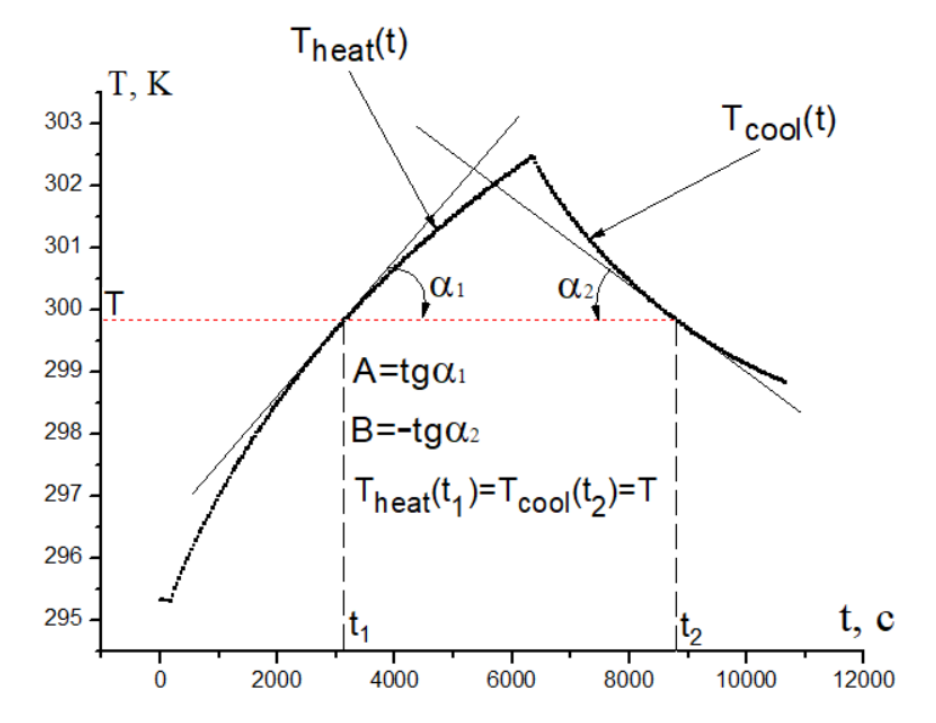
\includegraphics[width=0.6\textwidth]{img/diff_method.png}
    \end{figure}
    \begin{center}
        Рис. 2.
    \end{center}

    Следует иметь в виду, что определение величины $B$ на кривой охлаждения $T_{cool}(t)$ необходимо производить на участках кривой достаточно далеких от момента выключения нагревателя, после того как в калориметре закончатся переходные процессы «переполюсовки» тепловых потоков. Корректный интервал времени для определения В можно определить экспериментально из кривой $T_{cool}(t)$, спрямляя ее в координатах ($ln \frac{T_{cool} - T_{\text{к}}}{T - T_{\text{к}}}$, $t$) , после чего исключить из рассмотрения начальный нелинейный участок:

    \begin{figure}[ht]
        \centering
        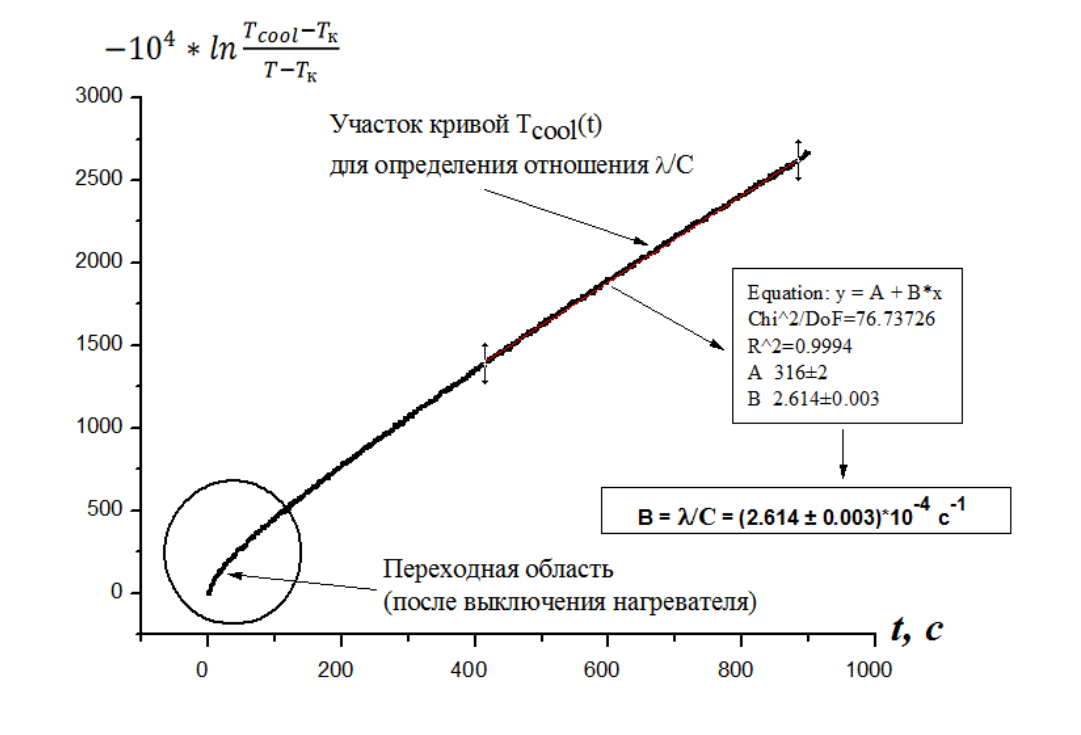
\includegraphics[width=0.6\textwidth]{img/not_lin_fragment.png}
    \end{figure}
    \begin{center}
        Рис. 3.
    \end{center}


\section{Приложение Б. Оценка погрешности измерения температуры и определение мощности нагревателя калориметра}

    Главная проблема калориметрического метода измерения теплоемкости – измерение температуры тела при его нагревании. В процессе нагревания температура тела неравномерно распределена по его объему. Из-за явления теплопроводности на поверхности тела она всегда выше. Термометр сопротивления, используемый в работе, измеряет температуру близкую к поверхности. Для минимизации погрешности в определении температуры важно, чтобы максимальная разница температур внутри тела и на его поверхности была как можно меньше. Ниже, по известным литературным данным для коэффициентов теплопроводности $c$, плотности $\rho$, и удельной теплоемкости $C_{\text{уд}}$, приведена оценка коэффициентов температуропроводности $k$ железа, алюминия, латуни, меди при стандартных условиях.
    
    Коэффициенты температуропроводности:

    \vspace{1 em}
    
    Железо (Fe):    $k = \frac{\text{\textchi}}{\rho}C_{\text{уд}} = 80,4/7870*460=2.221*10-5 \text{м²/с}$
    
    Алюминий (Al):  $k = \frac{\text{\textchi}}{\rho}C_{\text{уд}} = 237/2700*902.5=9.726*10-5 \text{м²/с}$
    
    Латунь (Cu+Zn): $k = \frac{\text{\textchi}}{\rho}C_{\text{уд}} = 121/8730*400=3.465*10-5 \text{м²/с}$
    
    Медь:           $k = \frac{\text{\textchi}}{\rho}C_{\text{уд}} = 401/8933*384.2=11.684*10-5 \text{м²/с}$
    
    \vspace{1 em}
    
    Исходя из величин и характерных размеров, можно оценить среднее время выравнивания температуры в исследуемых образцах и медной рубашке калориметра:

    \vspace{1 em}
    
    Железо (Fe):    $t \sim L^2/k = 0.022/2.221*10-5=18$ с
    
    Алюминий (Al):  $t \sim L^2/k = 0.022/9.726*10-5=4$ с
    
    Латунь (Cu+Zn): $t \sim L^2/k = 0.022/3.465*10-5=12$ с
    
    Медь:           $t \sim L^2/k = 0.032/11.684*10-5=11.7$ с

    \vspace{1 em}
    
    При требуемой точности в определении температуры тела, полученные оценки позволяют подобрать необходимую мощность нагревателя. Для данной работы вполне разумно, чтобы максимальная разница температур внутри тела и на его поверхности не превышала точность определения температуры терморезистора с помощью омметра, то есть не более $0.15 \celsius$. Тогда мощность нагревателя должна быть такова, чтобы за характерное время выравнивания температур ($~20 c$), температура на его поверхности возрастала не более, чем на $0.15 \celsius$. Подбор мощности нагревателя по данной методике для используемого в работе калориметра дает величину необходимой мощности $P \leq 6$Вт.

\section{Приложение В. Ход работы}

    \subsection*{Охлаждение калориметра}
    
    Вставили в калориметр охлаждённый латунный конус. Через 4 минуты после того, как температура в калориметре начала медленно расти, вынули латунный конус, вернули его в ёмкость с охлаждённой водой. Подождали ещё 3 минуты. Калориметр охладился примерно на $5 \celsius$.

    \subsection*{Определение зависимости сопротивления терморезистора от времени при нагревании пустого калориметра}
    
    Включили нагреватель. После того, как температура в калориметре превысила комнатную температуру на $7 \celsius$, отключили цепь спирали нагревателя.

    \subsection*{Определение зависимости сопротивления терморезистора от времени при охлаждении пустого калориметра}

    Проследили за температурой калориметра при его охлаждении. Когда она уменьшилась на 2 градуса по сравнению с максимальной, перешли на следующий этап.

    \subsection*{Охлаждение калориметра}

    Охладили калориметр до температуры на $5 \celsius$ ниже комнатной при помощи охлаждённого латунного конуса. 
    
    \subsection*{Определение зависимости сопротивления терморезистора от времени при нагревании калориметра с образцом алюминия}
    
    Вставили в калориметр исследуемый конус из алюминия и включили нагреватель. Нагревали систему "калориметр - алюминиевый конус", пока её температура не превысила комнатную на $7 \celsius$. Затем выключили нагреватель.

    \subsection*{Определение зависимости сопротивления терморезистора от времени при охлаждении калориметра с образцом алюминия}

    Проследили за температурой калориметра с алюминиевым конусом при его охлаждении. Когда она уменьшилась на 2 градуса по сравнению с максимальной после нагревания, перешли на следующий этап.

    \subsection*{Определение зависимости сопротивления терморезистора от времени при нагревании и последующем охлаждении калориметра с образцом титана}

    Повторили процессы нагревания и охлаждения, как это было сделано для калориметра с алюминиевым конусом, поместив в калориметр конус из титана.

    \subsection*{Окончание измерений}

    Останавливаем запись в программе. Сохраняем файлы с данным.

\section{Приложение Г. Расчёт теплоёмкости пустого калориметра}
    Построили  график зависимости температуры от времени для пустого калориметра:
    \begin{figure}[ht]
        \centering
        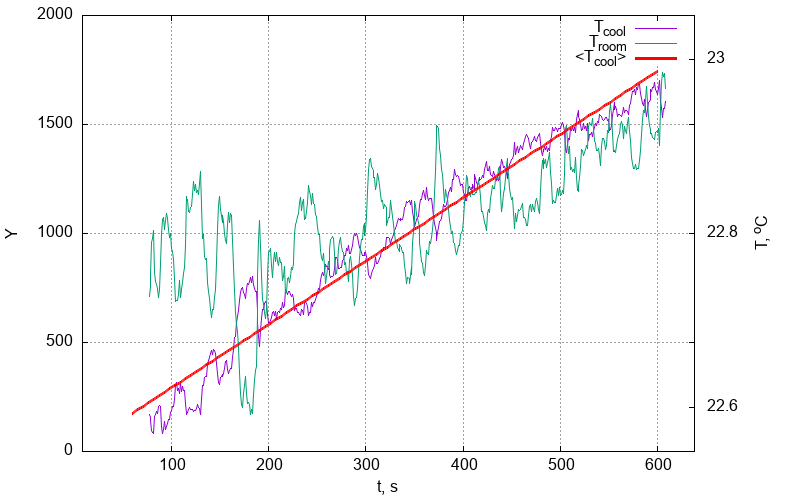
\includegraphics[width=\textwidth]{img/T_cool_1.png}
        \begin{center}
            Рис. 3 - График охлаждения пустого калориметра
        \end{center}
    \end{figure}\textbf{}

    Из графика получили $\lambda/C = (2.806\pm0.024)*10^{-4}\textrm{с}^{-1}$. Подставив это отношение в следующую формулу, нашли $\lambda$:
    $$T_{heat}(t) = \frac{P}{\lambda}(1-e^{-\frac{\lambda}{C}t})+T_k$$
    $$\lambda = 0.185 \pm 0.013, $$
    
    С помощью $\lambda$ вычислили теплоемкость $C$:
    $$C_0 = 659.3 \pm 46.5\frac{\textrm{Дж}}{\textrm{К}}, \quad \sigma_{C_0}=7 \% $$

    В расчёте использовалось, что мощность нагревателя $27.1*0.226 = 6.125\pm0.037$ Вт, так как напряжение нагревателя = $27.1\pm0.1$ В, сила тока = $0.226\pm0.001$ А.

\section{Приложение Д. Список литературы}

1. Титан. Мини-справочник по химическим веществам (3340 веществ)
https://xumuk.ru/spravochnik/232.html